\begin{figure}[htbp]
	\centering
	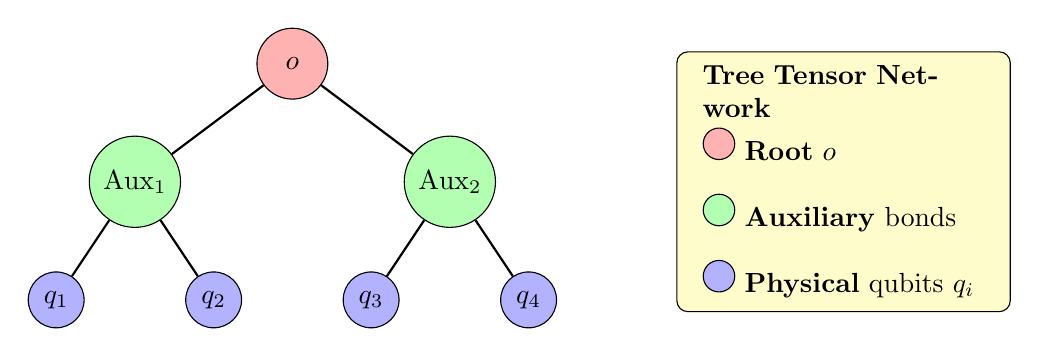
\begin{tikzpicture}[scale=1]
		\begin{scope}
			\node[draw, circle, fill=red!30, minimum size=0.9cm] (root) at (0,3) {$o$};
			\node[draw, circle, fill=green!30, minimum size=0.8cm] (aux1) at (-2,1.5) {Aux$_1$};
			\node[draw, circle, fill=green!30, minimum size=0.8cm] (aux2) at (2,1.5) {Aux$_2$};
			\node[draw, circle, fill=blue!30, minimum size=0.7cm] (q1) at (-3,0) {$q_1$};
			\node[draw, circle, fill=blue!30, minimum size=0.7cm] (q2) at (-1,0) {$q_2$};
			\node[draw, circle, fill=blue!30, minimum size=0.7cm] (q3) at (1,0) {$q_3$};
			\node[draw, circle, fill=blue!30, minimum size=0.7cm] (q4) at (3,0) {$q_4$};

			\draw[thick] (root) -- (aux1);
			\draw[thick] (root) -- (aux2);
			\draw[thick] (aux1) -- (q1);
			\draw[thick] (aux1) -- (q2);
			\draw[thick] (aux2) -- (q3);
			\draw[thick] (aux2) -- (q4);
		\end{scope}

		\begin{scope}[xshift=7cm]
			\node[draw, rounded corners, fill=yellow!20, text width=4cm, align=left] (legend) at (0,1.5) {
				\begin{tabular}{p{3.5cm}}
					\textbf{Tree Tensor Network}                                                                            \\[0.4cm]
					\tikz\node[draw, circle, fill=red!30, inner sep=1pt, minimum size=0.4cm] {}; \textbf{Root} $o$          \\[0.3cm]
					\tikz\node[draw, circle, fill=green!30, inner sep=1pt, minimum size=0.4cm] {}; \textbf{Auxiliary} bonds \\[0.3cm]
					\tikz\node[draw, circle, fill=blue!30, inner sep=1pt, minimum size=0.4cm] {}; \textbf{Physical} qubits $q_i$
				\end{tabular}
			};
		\end{scope}
	\end{tikzpicture}
	\caption{Tree Tensor Network (TTN) representation of multipartite states. Physical qubits ($q_i$) are at the leaf nodes, while auxiliary bonds (Aux$_j$) encode the entanglement geometry. The bond dimension $\chi$ controls the entanglement rank across each cut.}
	\label{fig:tree-tensor-network}
\end{figure}
